\section{Motivation}
%5) Our Approach: Briefly
In this paper, we present and evaluate \projectname{}, a system to prevent dangling pointers during run-time. \projectname{} uses metadata management framework to track metadata associated with memory objects. We use LLVM static transformation pass to insert run-time function calls. Our design is based on per-Thread per-Object data structure. Thereby, it removes need for thread synchronization. This lock-less design is highly efficient in heavily multi-threaded applications like, Web Servers. \\
 
This paper has following contribution,
\begin{itemize}
\item We evaluated effectiveness of \metalloc{} framework by implementing dangling pointer prevention. Design is similar to \cite{FreeSentry}. We show that thread synchronization may lead to huge degradation.
\item We propose \projectname{}, a unique lock-less system design to invalidate dangling pointers during run-time.
\item We implemented and evaluated \projectname{} on SPECint2006 CPU benchmarks and, widely used Web Servers (i.e. httpd, nginx and, lighttpd).
\item We evaluated \projectname{} for correctness on recently discovered use-after-free(and double-free) vulnerabilities.
\end{itemize}

This paper is organized as follows. Section II shows the effectiveness of \metalloc{} framework for preventing dangling pointers. Section III discusses our novel lock-less \projectname{} design. Also, it discusses design decision criteria and parameters. Section IV presents \projectname{} implementation and issues faced. Next, Section V evaluates \projectname{} in terms of performance and correctness. Related work is discussed in Section VI. Finally, Section VII concludes our contribution.

%1) Instrumentation phase
%2) Implementation of run-time using FreeSentry approach
%3) Comparison of with lock and without lock
%4) Need to go for other approaches

%1) Talk about dangling pointer creation.
Dangling pointer is created when the object is freed and pointer still has reference to it. Use of dangling pointer leads to undefined behaviour, mostly segmentation fault. Normally, developers set pointers value to NULL after object free. Applications have NULL check which prevents invalid dereferencing of dangling pointers. However, manually this technique is not scalable (feasible) when multiple pointer copies are present. Thus, We need metadata to keep track of almost all pointers pointing to the object during run-time. \metalloc{} is an efficient metadata management framework implemented on top of custom allocator, \texttt{tcmalloc}. We first implemented a pointer tracking scheme similar to \freesentry{} using \metalloc{}. To maintain object-to-metadata mappings, \freesentry{} uses label based system whereas \metalloc{} uses \textit{metapage table} (a hash table). This data structure should efficiently retrieve metadata given any inbound address to the object. To retrieve pointer-to-object metadata, we use a hash-table called as pointer lookup table. Figure~\ref{fig:metalloc-freesentry} shows new pointer tracking scheme based on \metalloc{}.\\

%\begin{figure}[t]
%\center
%  \includegraphics[width=2.8in,height=2.4in,keepaspectratio]{figures/metalloc-%freesentry.eps}
  %\caption{ Dangling pointer detection scheme based on \freesentry{} using %\metalloc{}.}
 % \label{fig:metalloc-freesentry}
 % \vspace{-1em}
%\end{figure}

\textbf{Implementation.} We maintain per object a structure called as headnode. It contains a unique identifier (ID) that determines the liveness of the object, a lock to protect pointer list, a pointer to the doubly pointer list and a MAGIC field. MAGIC field is a XOR result of ID and a Constant. \metalloc{} allocates headnode for every possible object (Global, Stack and Heap). It initializes headnode with zero. \metalloc{} metadata retrieval function returns pointer to the headnode. This return value can be NULL, garbage or a valid headnode. Thus, validity of the object is confirmed using MAGIC field. Moreover, tracking for stack objects and pointers can be skipped during run-time using MAGIC field. Also, tracking of global objects (not pointers) are skipped  by reserving lower 16 bits of identifier only for the global objects. It is assumed that total number of global objects during a run remains constant and less than $2^{16}$.  \\

Pointer information is tracked in a structure called as ptrnode. Each ptrnode contains, pointer address to invalidate, pointer value to check if pointer still points to the object, object ID in which pointer resides to check the validity of the pointer object, backward and forward pointers to iterate through doubly list.
Pointer lookup table gives mapping from pointer address to the pointer information. Each $8$ byte pointer contains a slot in the pointer lookup table. As size of pointer lookup table is limited, collision is handled through chained doubly linked list. When number of pointer traces increases, length of doubly linked list increases. Application runtime overhead increases dramatically when linked list traversal increases. Thus, pointer lookup table size should be selected wisely. \\

%2) Static instrumentation
\textbf{Static Instrumentation.} We use LLVM-based static instrumentation to insert run-time tracking functions. We have not instrumented any allocation (malloc, calloc, realloc, new) and deallocation (free, delete) calls. \metalloc{} provides a way to insert hook before or after allocation(deallocation routine). We have enabled hook after allocation routine and before free routine. These hooks initialize metadata and invalidate pointers from pointer list, respectively. We are only interested in pointer assignments. 
$$ store\ rhs,\ lhs $$
We wrote a function pass to track interested store LLVM IR instructions. We track only those store instructions where \textit{rhs} is a pointer type. Stack pointers are live only for the function scope. Also, we are not tracking stack objects. We conservatively filter out stores when \textit{lhs} or \textit{rhs} is a stack object. Moreover, incorrectly instrumented stack objects and address are skipped during run-time. We also skip stores when \textit{rhs} is a global object, a function pointer or a constant null pointer. We insert run-time tracking routine after store instruction in this design. However, in \projectname{} we insert it before store instruction. This is to check the old value of the pointer. \\

\textbf{Backward Compatibility.} Pointer invalidation by value NULL can break application backward compatibility. Many applications use freed object address as a numerical value to calculate relative offset or number of unit size elements. Setting pointer value to NULL will result into incorrect and undefined behaviour. To solve this problem, we invalidate pointer value by setting the most significant bit to $1$. On Linux $64$-bit this invalid address results into kernel address space. Next, some pointers can point out-of-bound. STL vector in C++ stores three fields, $1)$ Start of array $2)$ Next empty location in the array $3)$ End of array. Here, End of array points to one byte off the object bound. We register pointer by using pointer value to find the metadata. Thus, off-by-one object address will end up registering pointer into wrong object's metadata. To solve this problem, we increase the size of the requested memory during allocation by $1$. Also, we found a weird pointer usage in $gcc$. SPECint2006 $gcc$ allocates a memory and stores allocated address minus some constant value into the pointer. Registration of this pointer ends up in wrong object's metatdata. We handled this as a special case during static instrumentation. We register object root pointer when \textit{rsh} is GEP LLVM instruction and GEP indices operand is negative or SUB LLVM instruction. \\

%\begin{figure}[t]
%\center
%  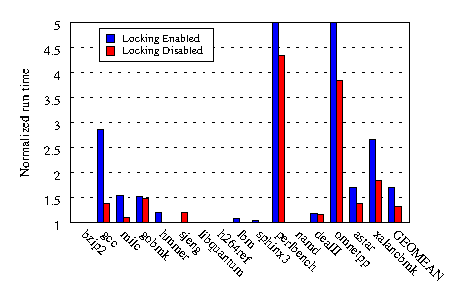
\includegraphics[width=3in]{plots/metalloc_freesentry.eps}
%  \caption{SPECint2006 performance overhead of dangling pointer prevention using %\metalloc{}. Locking enabled represents with thread synchronization and Locking %disabled represents without thread synchronization.}
%  \label{fig:metalloc-freesentry-graph}
%  \vspace{-1em}
%\end{figure} 

\textbf{Evaluation.} We instrumented SPECint2006 benchmarks with above pointer detection scheme. Safestack option is enabled for baseline numbers. \metalloc{} is implemented with \texttt{tcmalloc} custom dynamic memory allocator. We performed experiments on 64-bits CentOS Linux with Intel Xeon CPU E5-2640 v3. Figure~\ref{fig:metalloc-freesentry-graph} shows SPECint2006 runtime overhead with and without thread synchronization. With locking enabled, \texttt{perlbench} and \texttt{omnetpp} has normalized runtime degradation of more than $5x$ ($12x$ and $7x$ respectively). With thread synchronization, runtime overhead compared to baseline-safestack is $69.6$\% and without thread synchronization is $33.2$\%. We have used pthread mutex per memory object and a global pthread read-write lock for pointer lookup table protection. Also, pthread spinlock is used for assigning object identifiers. Out of three locks, pointer lookup table is highly contented. So, locking contributes huge performance degradation. \freesentry{} experiments only with single threaded applications. It has used no locks. We cannot directly compare performance of our design with \freesentry{}. Because, number of instrumentation and implementation may differ in both design. Moreover, \dangnull{} which uses pthread mutexes to protect its internal data structure has on average runtime overhead of $80$\%. Locking overhead is one of the reason in \dangnull{}. This problem has motivated to go for \projectname{}, a novel lock-less system to prevent dangling pointers in multi-threaded application.
